%MRC5Dec2102 Added Venture Requirements suggestion.
%Design Requirements Chapter
\chapter{Design Requirements}
\label{sec-requirements}

\begin{remark} \color{blue}
Articulating design requirements is a critical task for a team that starts with a broad problem and needs to determine \emph{what they should design}. After need-finding, and technical and user benchmarking, the team proposes a {\em class of design solutions} that fulfill {\em requirements}\, associated with the problem. In the Fall document, the initial Requirements Definition is one of the first items of real value that teams can deliver to sponsors.

As the design process continues, requirements become more concrete and detailed. New {\em de facto} \, requirements are discovered and documented. Ultimately, competing designs are evaluated with respect to the requirements. If you can't tell whether a design satisfies the requirements, the requirements are too vague.


It is suggested to follow the procedure introduced in Fall quarter lectures and the Paper Bicycle Documents for defining and organizing requirements:\\
 \url{http://wikibox.stanford.edu:8310/12-13/Public/Fall2012-2013/Week2_2-4Oct/}

\normalcolor \end{remark}

%This table can  be copied & pasted in your document. The fussy formatting is already set up correctly.
%To get wrapped text, you have use p{} and specify paragraph widths (total < 148mm)
\begin{table}
\color{blue}
  \begin{tabular}{| p{44mm} | p{49mm} | p{42mm} |}   %3 columns, wrapped text
  \hline
  Requirement & Metrics & Rationale \\
  \hline
  \emph{What is the issue?} & \emph{What target values are we looking for?} & \emph{Why is this important?}\\
    \hline
  a brief description of what the requirement or objective is & 
  measurable quantities associated with requirement (how one knows if a design satisfies the requirement) &
  the  reasons why the it is important or valid \\

% This example table can be copied and pasted with the text adjusted to meet your needs. &
% Each column is separated by an ``\&'' sign. The text entries can wrap to more than one line if needed. &
% Each row is separated by two backslashes and an optional horizontal line. \\
    \hline
  \end{tabular}
\caption[Three column requirements format]{Three column format suggested for requirements (One can make a separate table for each cluster of related requirements).}
	\label{threecolumnreqs}  %Tag for referring to table
\normalcolor
\end{table}

\begin{remark} \color{blue}
The remainder of this section contains sample requirements (not an exhaustive set but enough to give an idea) from Autodesk Fall 2007-08 \cite{Autodesk2008Fall} and Audi Fall 2008-09 \cite{Audi2009Fall}.
\normalcolor \end{remark}

%%%%%%%%%%%%%%%%%%%%%%%%%%%%%%%%

\section*{Introduction}

The Autodesk collaboration tool must enhance communication between groups of distributed engineers as they engage in brainstorming.  We have focused on enabling this collaboration via tools that:

\begin{itemize}\tightlist
\item Enable users to communicate naturally and through multiple channels.
\item Enable the team to better utilize their teammates, be they local or distant.
\item Capture the information that was presented.
\end{itemize}

Our benchmarking and prototyping efforts have led to a more detailed definition of what the product needs to be in order to successfully achieve this.  The requirements address what the product functionally needs to do and what it physically needs to be. Because of the wide range of functional opportunities that exist for the product, few physical restrictions are imposed at this stage in the design. 

\section{Functional Requirements}
\label{sec:functionalreqs}

\begin{table}[!h]
	\centering
		\begin{tabular}{| p{42mm} | p{42mm} | p{51mm} |}
		\hline
		\textbf{Requirement}	& \textbf{Metrics} & \textbf{Rationale}\\
		\hline
The product will balance the number of interactions in distributed design meetings among the team members. &	Interactions are questions or statements that develop a concept. The total number of interactions per person during a design meeting will be called $n_{i}$. The solution must reduce the standard deviation of $n_{i}$ between team members as compared to the closest publicly-available competing product.	& The number of times someone interacts in a meeting is one measure of engagement. Brainstorming is a highly social process which thrives on the input from a variety of perspectives. By effectively improving the communication between distributed teams, team members will be more engaged and participate more.\\
\hline
		\end{tabular}
	\caption{Requirement for improved communication}
	\label{tab:mediums1}
\end{table}

\begin{table}[!h]
	\centering
		\begin{tabular}{| p{42mm} | p{42mm} | p{51mm} |}
		\hline
		\textbf{Requirement}	& \textbf{Metrics} & \textbf{Rationale} \\
		\hline
The solution must transmit sound at close to the rate of normal conversation. &	The listener must hear the speaker with less than 0.3 seconds lag.	& Audio latency creates a sense of distance. Mobile phone to mobile phone conversations have an average latency of 0.3 seconds, which is noticeable but not disruptive. \\ \hline
Users can capture drawings to share with distributed teammates that are legible. &	Input device must be able to resolve a drawing at 50 points per inch (specifically, they must capture 50 percent contrast modulation at this frequency). &	Drawings by mechanical pencil and ball point pens typically have lines of 0.5mm thickness, which translates to a resolution of 50 points per pinch (ppi).\\ \hline
Users will be able to capture drawings to share with distributed teammates without disrupting the flow of the discussion. & Drawings must be captured and sent within 17 seconds. This is assuming the input device is properly set and there are no external complications. &	We found through benchmarking that sketches are used primarily when describing a concept, and are of little use afterwards. The sketches must be captured and sent before the context of the discussion has changed. Seventeen seconds was found to be about the average comment length during brainstorming in our prototyping. \\ \hline
Users will be able to see the drawings clearly. &	Drawings must be displayed with a resolution of at least 72 ppi.&	The display must be able to resolve at least as a standard computer monitor.\\ 
\hline
		\end{tabular}
	\caption{Required mediums of communication for effective concept development}
	\label{tab:mediums2}
\end{table}

\begin{table}[!h]
	\centering
		\begin{tabular}{| p{42mm} | p{42mm} | p{51mm} |}
		\hline
		\textbf{Requirement}	& \textbf{Metrics} & \textbf{Rationale} \\
		\hline
The tool must be able to be started up quickly for impromptu meetings.	& It must be able to be started in less than 40 seconds. This time is calculated from the moment someone decides to start the system, to the point when the tool is ready to use, with full functionality. If the solution requires use of personal laptops, assume these are already booted up. & Our benchmarking has shown that collaboration tools can fall into disuse if it requires a lengthy setup time. This amount of time is within the range of initiation times for multiple popular conferencing solutions. \\ \hline

	\end{tabular}
	\caption{Social requirements for effective design meetings}
	\label{tab:mediums3}
\end{table}



\newpage

\subsection{Functional constraints}

\begin{table}[!h]
	\centering
		\begin{tabular}{| p{44mm} | p{49mm} | p{42mm} |}
		\hline
		\textbf{Requirement}	& \textbf{Metrics} & \textbf{Rationale} \\
		\hline
		The bandwidth required must not be prohibitive to standard engineering offices.	& The product will require less than 100 Mbps.& The population of potential users would dramatically decrease if the product required more connectivity than a T1 line, which is typically around 100 Mbps.\\ \hline
			\end{tabular}
	\caption{Functional constraints}
	\label{tab:fconstraints}
\end{table}


\subsection{Opportunities}

\begin{itemize}\tightlist
\item Utilize existing tools. There are many collaboration and input  tools that exist out there. Our product does not need to be a replacement for them. It could potentially supplement them.
\item Offer new lines of communication:
	\begin{itemize}\tightlist
 		\item Facilitate side conversations between distributed users.
 		\item Utilize the uncrowded channels offered by other senses than audio/visual, such as tactile.
\end{itemize}
\newpage
\item Be the moderator: 
\begin{itemize}\tightlist
 		\item Collect feedback from users directly, via voting, or indirectly. Enable the replacement of video, which conveys very little useful feedback during design meetings.
		\item Encourage the participants to be engaged by monitoring participation.
		\item Display feedback and participation to attendees non-verbally,potentially through the use of avatars.	
\end{itemize}
\item Allow for easier information capture and storage
\begin{itemize}\tightlist
 		\item One button information capture
		\item User-driven archiving
\end{itemize}
\item Assist user communication in non-native languages.
	\begin{itemize}\tightlist
 		\item Audio buffering
 \end{itemize}
\item The product should be accessible
\begin{itemize}\tightlist
\item Usable for low bandwidth connections for 
\item Be fast to setup.
\item Able to be setup within a typical conference room.
\end{itemize}
\end {itemize}

\subsection{Assumptions}
\begin{itemize}\tightlist
\item Each user has, and is able to use:
\begin{itemize}\tightlist 
\item a personal laptop
\item a mouse
\item a microphone
\end{itemize}
\item Users will speak with a volume of at least 30 dB, as measured when 1 meter from the microphone.
\end{itemize}

%%%%%%PHYSICAL REQUIREMENTS%%%%%%%%%%%
\section{Physical requirements}
\label{sec:physicalreqs}

\color{blue}
For variety, here is a requirements table from an Audi fall document \cite{Audi2009Fall} done in MS Word and pasted as PDF into Latex. Notice that the fonts are scalable if you zoom in.
\normalcolor

\begin{table}[h]
	\centering
		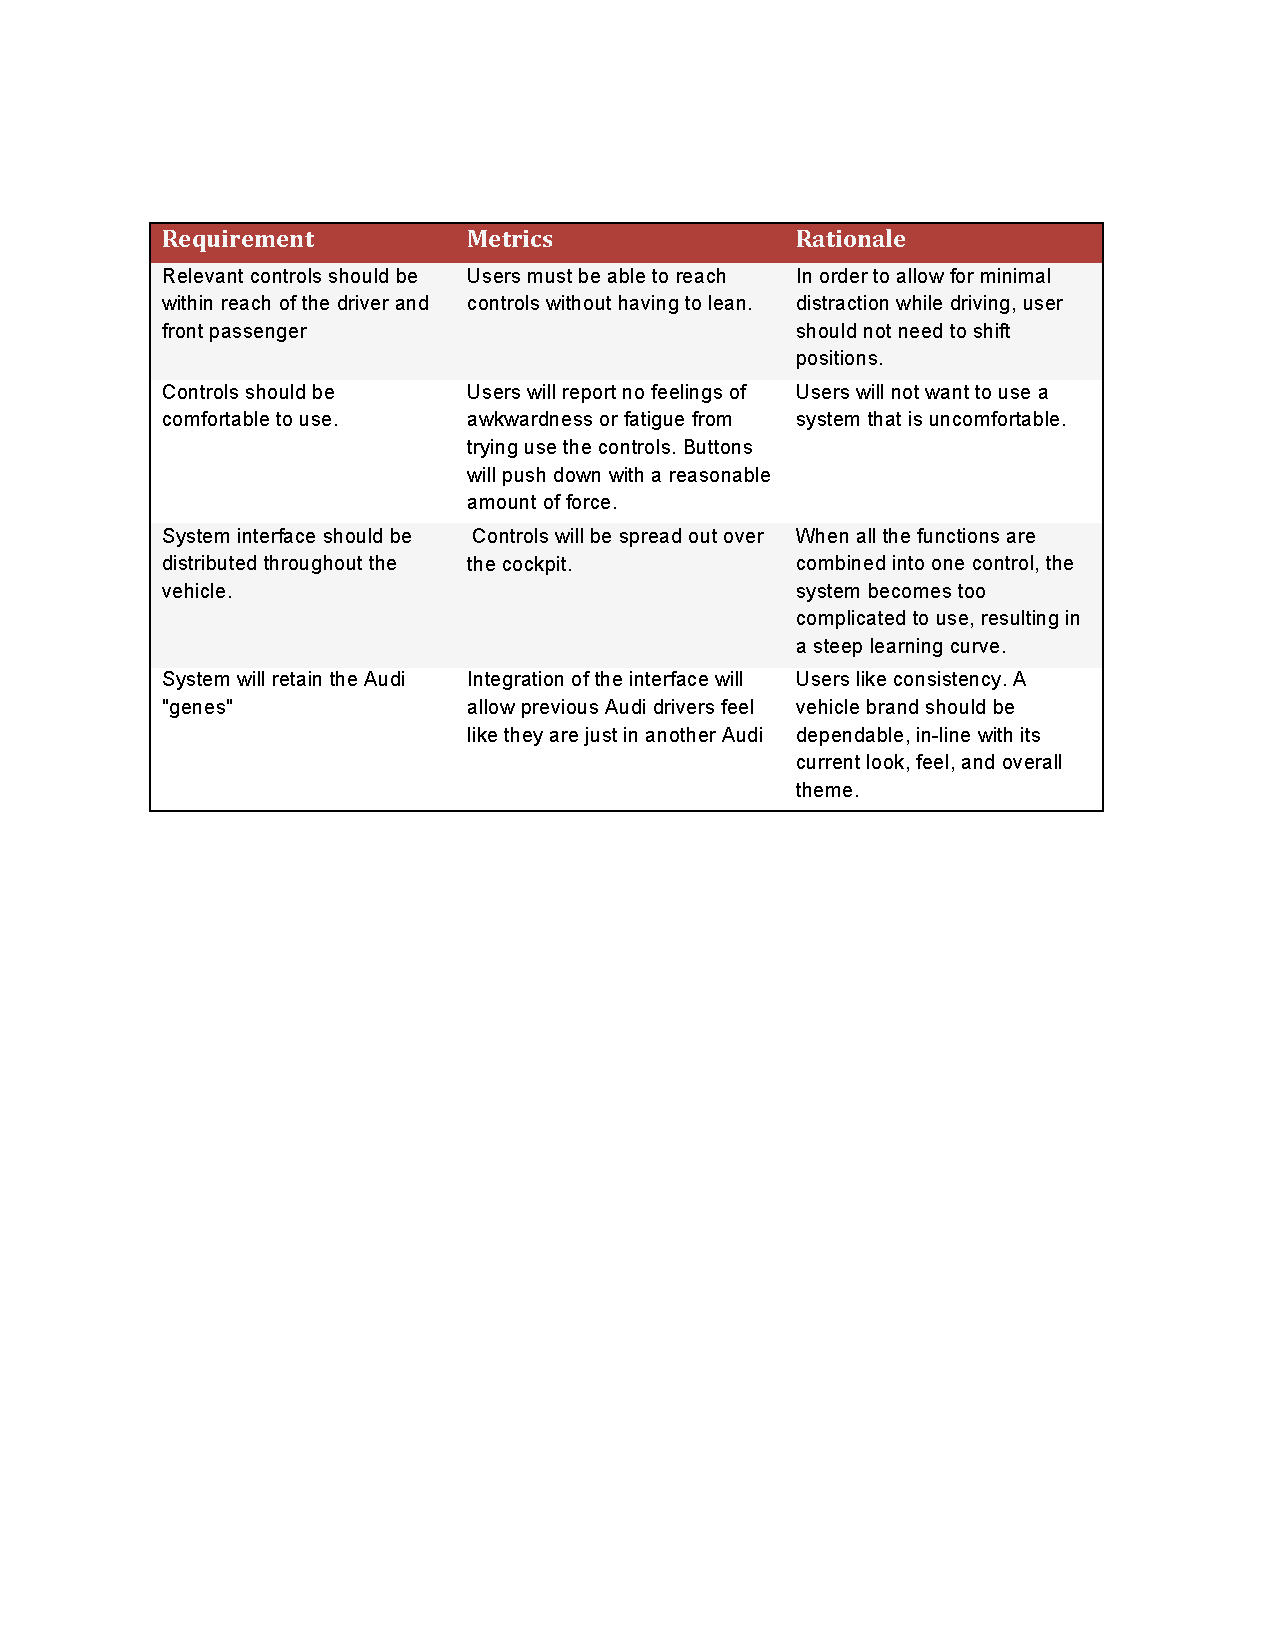
\includegraphics[width=\textwidth]{Figures/Ch3/Audi08PhysReqs.pdf}
	\caption{Physical Requirements from Audi 2008-09}
	\label{tab:physical-requirements}
\end{table}

\subsection{More physical requirements}
\label{sec:morephysical}

\color{blue}
Here is an example of a Physical Requirements table from a spring document. The 4th column is probably not appropriate for Fall. This example is include to show how one can make a long table that spans multiple pages.
\normalcolor

%%Example of a long  table using supertabular and tablefirsthead
%%
\begin{center}
\tablefirsthead{%
\hline
\textbf{Requirements} & \textbf{Metric} & \textbf{Rationale} & \textbf{Requirements met?}\\
\hline}
\tablehead{%
\hline
\multicolumn{4}{|l|}{\textit{\small{continued from previous page}}}\\
\hline
\textbf{Requirements} & \textbf{Metric} & \textbf{Rationale} & \textbf{Requirements met?}\\
\hline}
\tabletail{%
\hline
\multicolumn{4}{|l|}{\textit{\small{continued on next page}}}\\
\hline}
\tablelasttail{\hline}
\bottomcaption{This physical requirements table is from a spring document to show splitting across pages and addition of a 4th column regarding whether design meets the requirements}
\begin{supertabular}{| p{32mm} | p{37mm} | p{33mm} | p{33mm} |}
\hline
Use limited force to activate mechanical mechanism(s) & Force required for activation is {\textless} 20 N & User should be able to operate system without excessive force & The design should fulfill this requirement, however final gas spring and seat securer installation and thereafter testing will confirm this\\
\hline
System is ergonomic & User should be able to operate all mechanisms 4 times in the span of 1/2 an hour without any serious exertion (no sweating, strained breathing, or muscle soreness) and should be able to use the system for 2 hours without muscle cramping or other physical afflictions & System should be physically comfortable to use for a long commute time & User testing needs to be performed; initial prototyping seems to show this is satisfied\\
\hline
System is durable and robust & Lasts at least 2 years of daily use and its structure cannot be significantly altered by an average man or woman applying a full impact force on structural elements of the module & As part of a PT system, all modules should be resistant to daily use by an average human and vandalism & Robust materials such as steel and actual public transport-quality seats and flooring has been used; needs to be tested\\
\hline
Parts can be easily replaced and easy to maintain, including easily cleaned and water resistant & Takes no more than 5 min for one person to replace parts of a single module; module can be fully cleaned in 15 minutes; module shows no signs of corrosion over its 2 year life span & PT parts see significant wear and it should be convenient to replace modules as necessary & Needs to be verified\\
\hline
Seat is comfortable & Seat is breathable (from fully soaked takes {\textless}15 to air dry) and has a high thermal conductivity (seat adjust to room temperature from a 20-degree difference in less than 5 minutes) & Commuter should have a pleasant commuting experience while seated & Good quality seats of actual public transportation quality have been procured and used\\
\hline
Module should be safe & There should be no pinch points, sharp points, or possibilities for latches or other physical mechanisms to fail & System should not cause any users bodily injury & Mechanisms have been designed to avoid pinch points; final verifications needed\\
\hline
System should be aesthetically pleasing & At least 80\% of surveyed users should react positively to the device forms & A pleasing system will encourage adoption and use & Visual language was established earlier on in the design phase; final aesthetic styling still needed upon final integration\\
\hline

\end{supertabular}
\end{center}

\section{Business requirements (or Venture requirements)}
\label{sec:venturereqs}

A new element in me310-global thinking for 2012-13 is to be more aware of the client�s business model.  This is not so much about designing a new business model as it is about business context awareness.  The main discussion of this business model belongs in chapter \ref{sec-development} as part of your benchmarking. Here is where you could note any particular requirements or ramifications  that it has for your design.





